\documentclass{beamer}
\usepackage[utf8]{inputenc}
\usepackage[T1]{fontenc}
\usepackage[english]{babel}
\usepackage{graphicx}
\usepackage{times}

\usetheme{AGH}

\title{Computational Intelligence project and laboratory summary}

\author[M. Nowotynski]{Matuesz Nowotynski}%TODO

\date[2018]{19.06.2018}

\institute[AGH]
{Faculty of EAIiIB\\ 
Department of Applied Computer Science
}

%\setbeamertemplate{itemize item}{\textbullet}

\begin{document}

{
\usebackgroundtemplate{
\includegraphics[width=\paperwidth]{titlepage}} % wersja angielska
%\usebackgroundtemplate{
\includegraphics[width=\paperwidth]{titlepagepl}} % wersja polska
 \begin{frame}
   \titlepage
 \end{frame}
}

%---------------------------------------------------------------------------


\begin{frame}
\frametitle{Multilayer perceptron}

\begin{itemize}
	\item Consists of at least three layers of non-linear perceptron nodes
	\item MLP very often called "vanilla" neural networks since they was first used in practice
	\item Uses backpropagation algorithm for learning
	\item Hard to create very deep networks because of vanishing gradient problem
\end{itemize}

\end{frame}

\begin{frame}
\frametitle{Multilayer perceptron -- my implementation}

\begin{itemize}
	\item Implementation create in C++17
	\item Each perceptron is separate object
	\item Perceptrons are using sigmoid activation function
	\item Input data was normalized using external software
\end{itemize}

\end{frame}
%---------------------------------------------------------------------------

\begin{frame}
\frametitle{MLP results on Iris data}
\begin{center}
	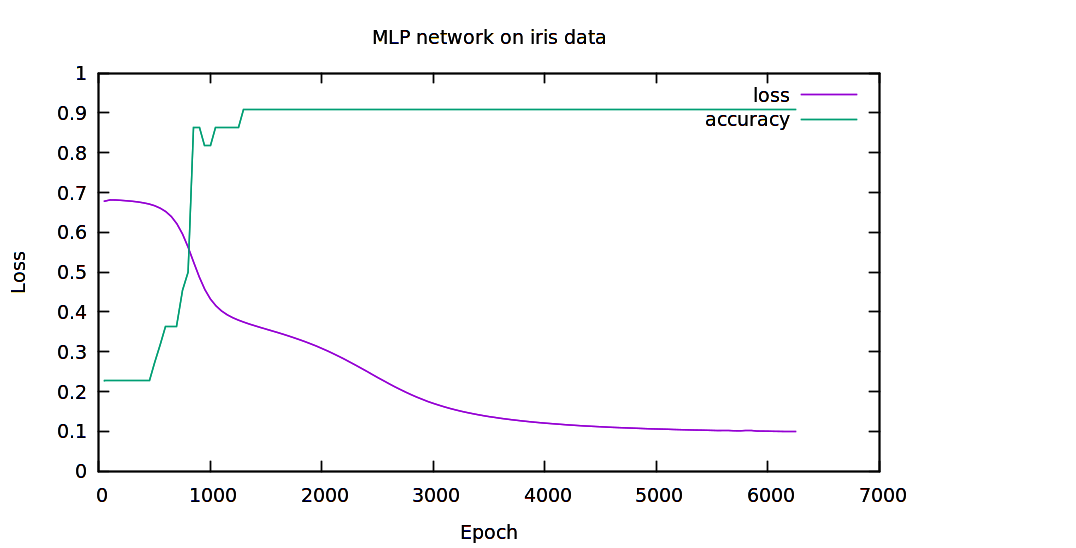
\includegraphics[width=\textwidth]{mlp_results}
\end{center}
\end{frame}

%---------------------------------------------------------------------------


\begin{frame}
\frametitle{Autoencoder}
\begin{center}
	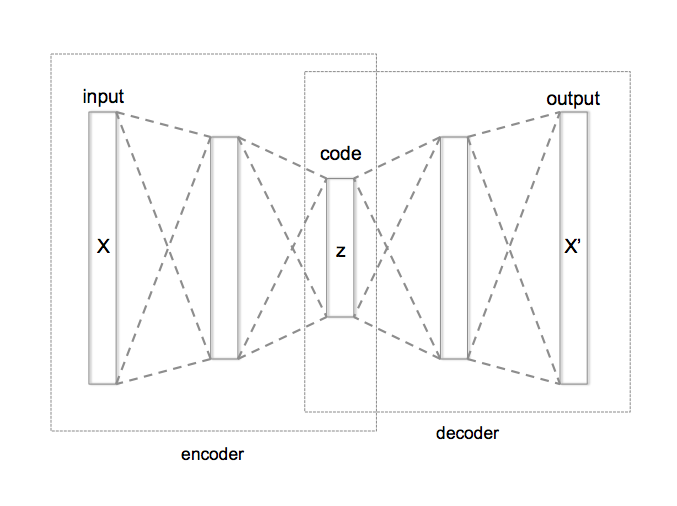
\includegraphics[width=0.7\textwidth]{Autoencoder_structure}
\end{center}
\end{frame}

%---------------------------------------------------------------------------

%\begin{frame}
%\frametitle{Autoencoder -- my implementation}
%\begin{itemize}
%	\item Based on MLP implementation
%\end{itemize}
%\end{frame}

%---------------------------------------------------------------------------

\begin{frame}
\frametitle{Autoencoder -- results on iris data}
	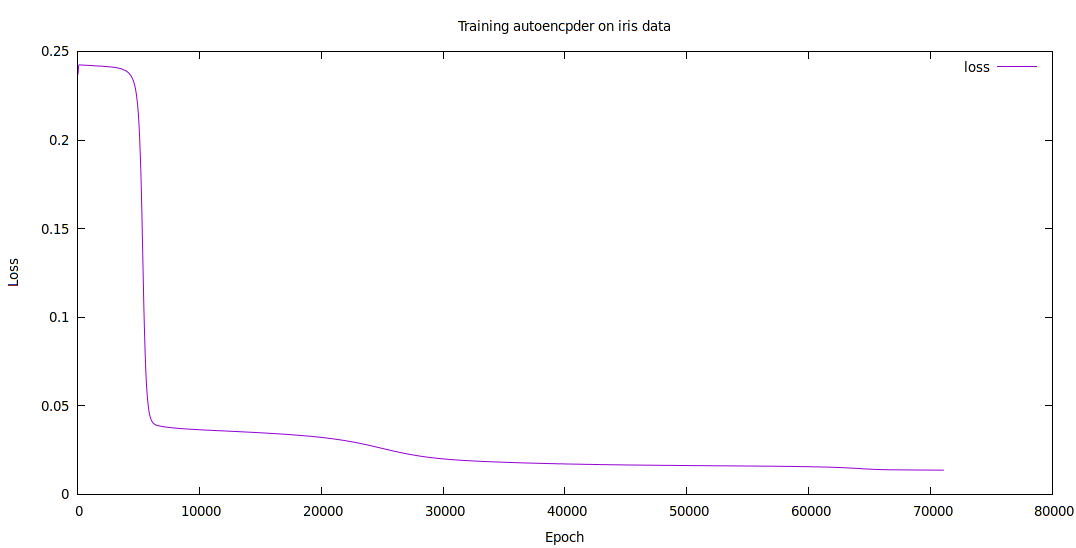
\includegraphics[height=0.65\textheight]{autoencoder}
\end{frame}

\begin{frame}
\frametitle{Autoencoder -- results on iris data}
	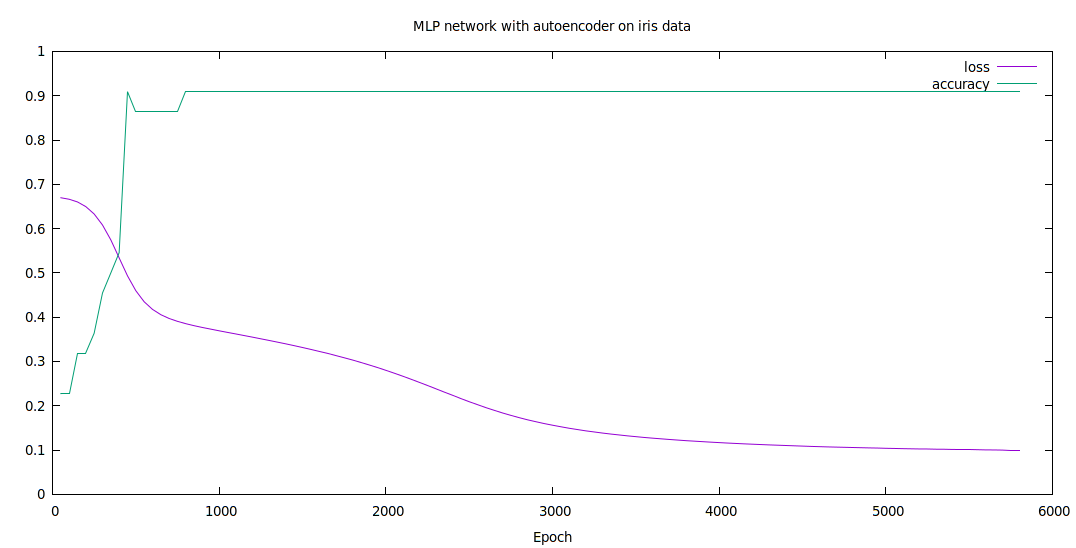
\includegraphics[height=0.65\textheight]{autoencoder_mlp}
\end{frame}

%---------------------------------------------------------------------------

\begin{frame}
\frametitle{AGDS}
\begin{itemize}
	\item AGDS -- Passive associative graph data structure
	\item useful for finding similar elements
	\item Implemented using SortedSet
\end{itemize}
\end{frame}


\begin{frame}
\frametitle{AGDS -- results}
Top similarities to Iris(5.0,2.0,3.5,1.0,2):
\begin{enumerate}
\item 1.000: Iris(5.0,2.0,3.5,1.0,2)
\item 0.966: Iris(5.0,2.3,3.3,1.0,2)
\item 0.953: Iris(4.9,2.4,3.3,1.0,2)
\item 0.932: Iris(5.5,2.4,3.7,1.0,2)
\item 0.927: Iris(5.1,2.5,3.0,1.1,2)
\item 0.921: Iris(5.5,2.4,3.8,1.1,2)
\item 0.916: Iris(6.0,2.2,4.0,1.0,2)
\item 0.915: Iris(5.7,2.6,3.5,1.0,2)
\item 0.906: Iris(5.5,2.3,4.0,1.3,2)
\item 0.891: Iris(5.5,2.5,4.0,1.3,2)
\end{enumerate}

\end{frame}
%---------------------------------------------------------------------------

\begin{frame}
\frametitle{Project -- CNN network for image classification}
\begin{itemize}
	\item Image classification
	\item Deep Convolutional neural network
	\item With residual path
\end{itemize}
\end{frame}

\begin{frame}
\frametitle{Mnist}
\begin{center}
	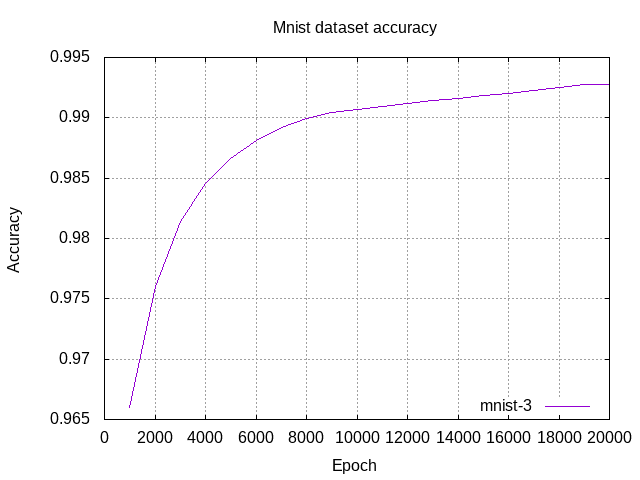
\includegraphics[height=0.45\textheight]{mnist-accuracy}
	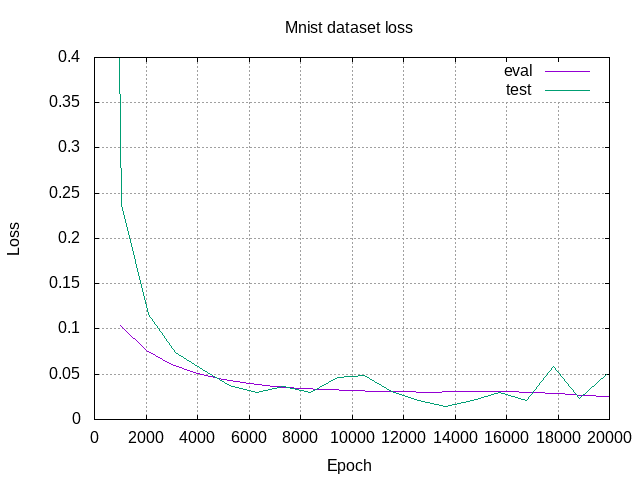
\includegraphics[height=0.45\textheight]{mnist-loss}
\end{center}
\end{frame}

\begin{frame}
\frametitle{Cifar}
\begin{center}
	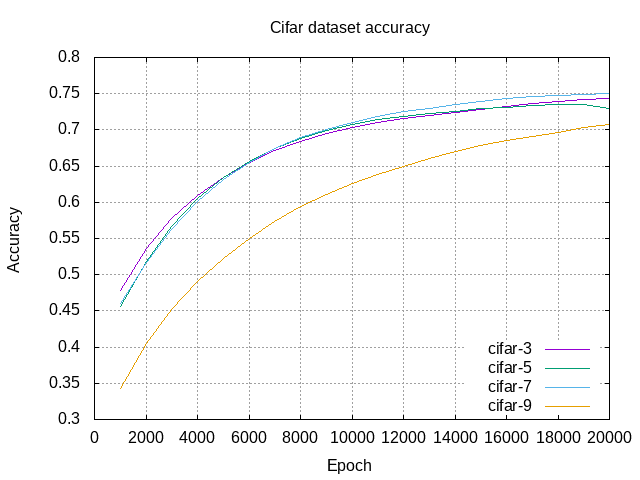
\includegraphics[height=0.45\textheight]{cifar-accuracy}
	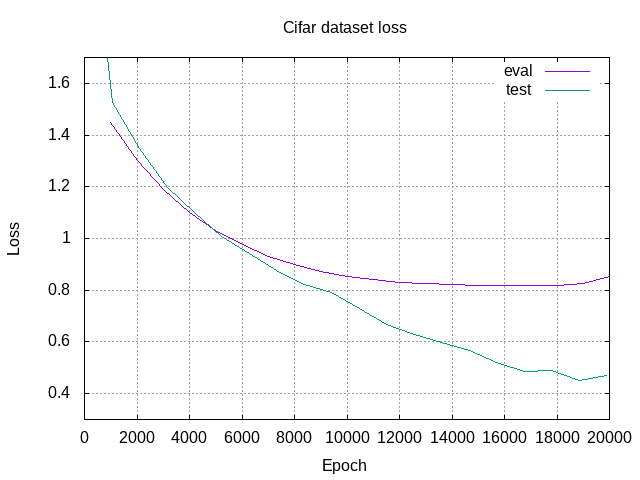
\includegraphics[height=0.45\textheight]{cifar-loss}
\end{center}
\end{frame}

\begin{frame}
\frametitle{Caltech}
\begin{center}
	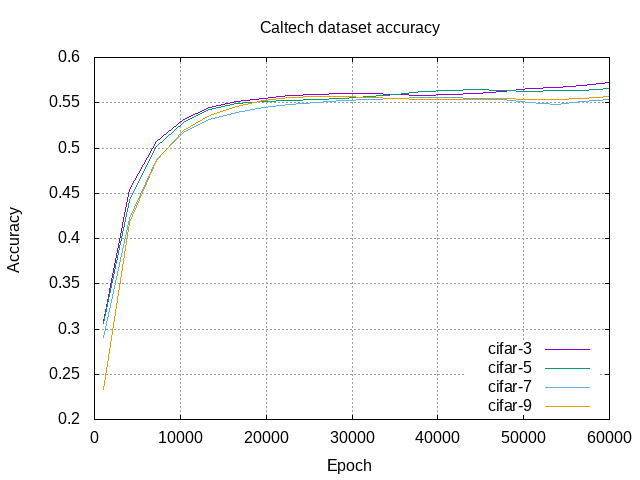
\includegraphics[height=0.45\textheight]{caltech-accuracy}
	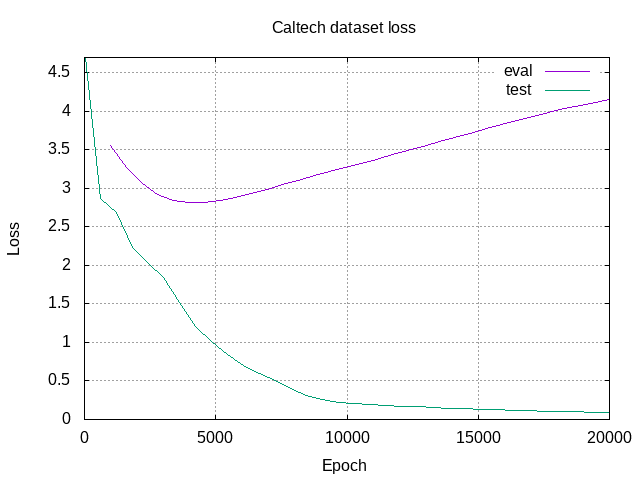
\includegraphics[height=0.45\textheight]{caltech-loss}
\end{center}
\end{frame}

\begin{frame}
\frametitle{Lessons learned}
\begin{itemize}
	\item Start with small network first
	\pause
	\item Know your data
\end{itemize}
\end{frame}

\end{document}

